\chapter{Path Optimization for Humanoid Walk Planning: an Efficient Approach}
\label{chap:path-optim}

This chapter deals with path optimization for humanoid walk planning
in cluttered environments. Under the assumption that the humanoid
robot will walk on a flat floor in a perfectly modeled static
environment, it presents a heuristic and efficient optimization method
that takes as input a path computed for the humanoid bounding box, and
produces a path where a discrete set of configurations is reoriented
using an A$^{*}$ search algorithm. A pattern generator is then used to
generate a trajectory that minimizes walking time. This method is
validated in various scenarios on the humanoid robot HRP-2.

\section{Motion Planning in the Configuration Space}
\label{sec:chap1-motion-planning}

The problem of motion planning is now well formalized in robotics and
several books present the various approaches
\cite{lato91,chos05,lava06}. One particularly useful concept is the
one of \emph{configuration space} {\cspace} \cite{loza83}, which is
the set of all configurations \config{} of a robot {\robot}; \config{}
is a vector comprised of the $n$ independent \emph{degrees of freedom
  (DoF)} that are sufficient to uniquely identify the full state of
the robot at each instant. {\cspace} defines then a manifold of
dimension~$n$. Some of the robot body positions can generate
(self-)collisions; the equivalent configurations will be said to be in
collision, and the set of all configurations in collision is denoted
by {\cobs} $\subset$ {\cspace}. Its complement is denoted by {\cfree}
and is called the \emph{free configuration space}. Using these
notations, we can redefine the motion planning problem as the answer
to the following question: is there a continuous path $P: [0,1]
\rightarrow$ {\cfree} that connects a start configuration \config{s}
to a goal configuration \config{g}, and what is it?

\subsection{Deterministic Algorithms}
\label{subsec:chap1-deterministic algorithms}

This question can be answered through the use of deterministic
algorithms; for a given number of tries, they will always compute the
same valid path $P$.

One class of algorithms, mainly developed in the past 30 years, relies
on representing {\cobs} explicitly in order to build a graph, also
called roadmap, that represents the connectivity of {\cfree}. Solving
the motion planning problem then boils down to a graph exploration to
connect \config{s} to \config{g}. A non-exhaustive list of these
methods includes cellular decomposition, Voronoi diagrams, visibility
graphs, and Canny's algorithm \cite{good04}.

Such algorithms offer the nice property of completeness, i.e.\ they can
always provide an answer to the motion planning problem as defined
previously. But while they work well for solving path planning
problems in low-dimensional configuration spaces, using them in
high-dimensional configuration spaces is either impossible by design,
or is computationally expensive, as building {\cfree} requires finding
its frontiers, and computation time is at best exponential with
respect to the dimension of {\cspace}.

Other approaches are inspired from real-time motion generation
techniques, such as the one detailed in \cite{khat85}, which consists
in assigning artificial attractive potentials on the goals, and
repulsive ones around the start configuration and the obstacles. The
robot is then subject to forces that will direct it from the start
configuration towards the goal configuration. However, because of the
locality of the planner, a path may be computed while not being a
solution to the path planning problem. This can happen in a maze-like
environment when a stable equilibrium point other than the goal
configuration is found (see Figure
\ref{fig:chap1-deterministic-algorithm}).

\begin{figure}
  \centering
      {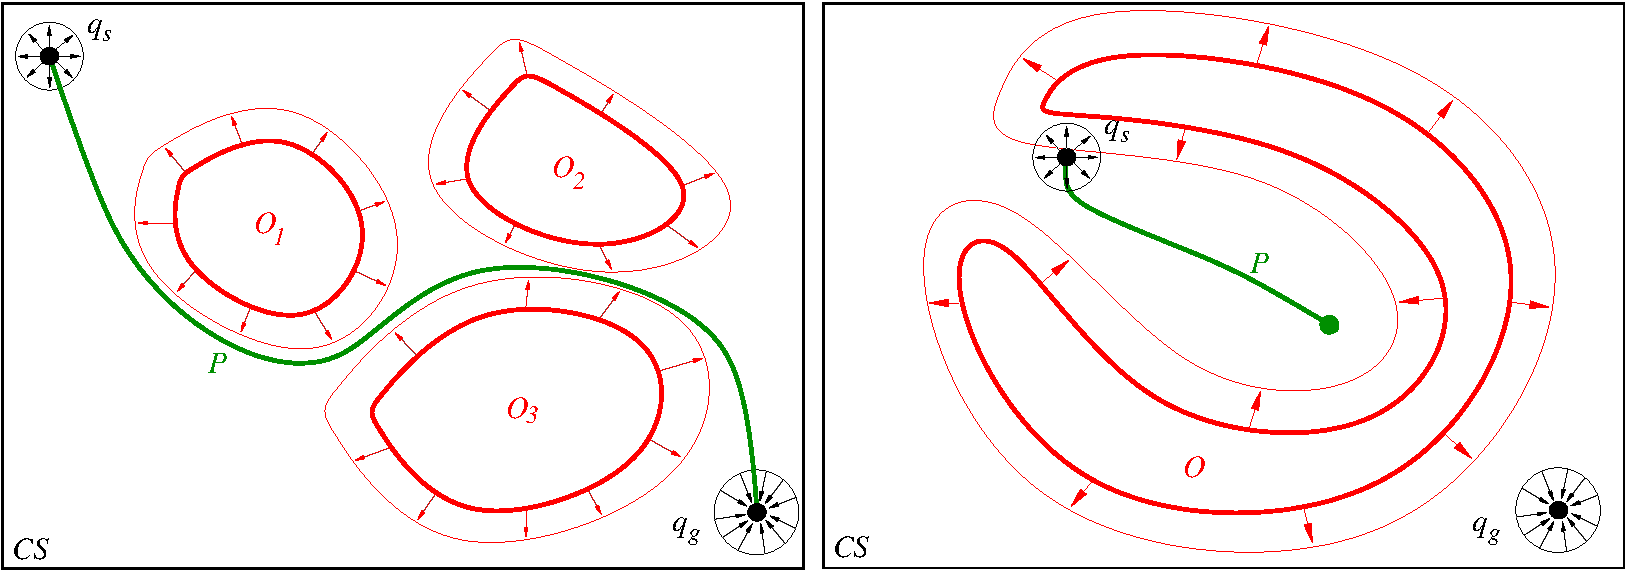
\includegraphics[width = \linewidth]
        {src/chap1-path-optimization/deterministic-algorithm.pdf}}
      \caption{Left: A valid path is computed by the deterministic
        algorithm. Arrows show the attractive and repulsive potential
        fields. Thin lines show the potential lines. Right: Example of
        problem where the stable local minimizer does not coincide
        with the goal configuration, which is the global
        minimizer. $P$ is thus not a solution to the path planning
        problem.}
      \label{fig:chap1-deterministic-algorithm}
\end{figure}

\subsection{Sampling-based Algorithms}
\label{subsec:chap1-sampling-algorithms}

Deterministic algorithms rapidly reach their limit when the
configuration space dimension rises above 4. Computation speed plays a
big part in choosing which algorithm to use for path planning
problems, as many applications require, or at least aim for, real-time
resolution. In this perspective, sampling-based algorithms, such as
Probabilistic Roadmaps (PRM) \cite{kavr96} or Rapidly-exploring Random
Trees (RRT) \cite{kuff00}, were developed in the past fifteen years.

Instead of trying to build an explicit representation of {\cfree},
sampling-based algorithms rely on approximating the connectivity of
{\cfree} through rejection sampling: random configurations \config{rand}
are sampled in {\cspace}, and efficient Boolean collision detection
techniques \cite{huds97, gott96} reject configurations that produce
collisions, keeping only configurations \config{} $\in$ {\cfree}.

The classic RRT algorithm, as presented in \cite{kuff00}, make use of
the Voronoi bias to efficiently explore {\cfree} and grow a random tree
in it. Each iteration of the algorithm attempts to extend the tree by
adding new vertices in the direction of a randomly selected
configuration \config{rand}. Algorithm~\ref{alg:chap1-rrt} shows the
pseudo-code of the RRT algorithm. It takes as input an initial
configuration \config{s} and grows a tree {\ctree} rooted in \config{s}.

\begin{algorithm}
\caption{\texttt{RRT}(\config{s})}
\label{alg:chap1-rrt}
\begin{algorithmic}
\STATE {\ctree}$.$Init$($\config{s}$)$
\FOR{$i$ = 1 to $K$}
\STATE \config{rand} $ \leftarrow $ Rand$(${\cspace}$)$
\STATE \config{near}$ \leftarrow $ Nearest$($\config{rand}$,${\ctree}$)$
\STATE Extend$(${\ctree}$,$\config{near}$,$\config{rand}$)$
\ENDFOR
\end{algorithmic}
\end{algorithm}

One way to make the RRT algorithm more efficient is to grow trees from
both the initial and goal configurations, see Figure
\ref{fig:chap1-rrt}. This was first proposed in \cite{kuff00}.

\begin{figure}
  \centering
      {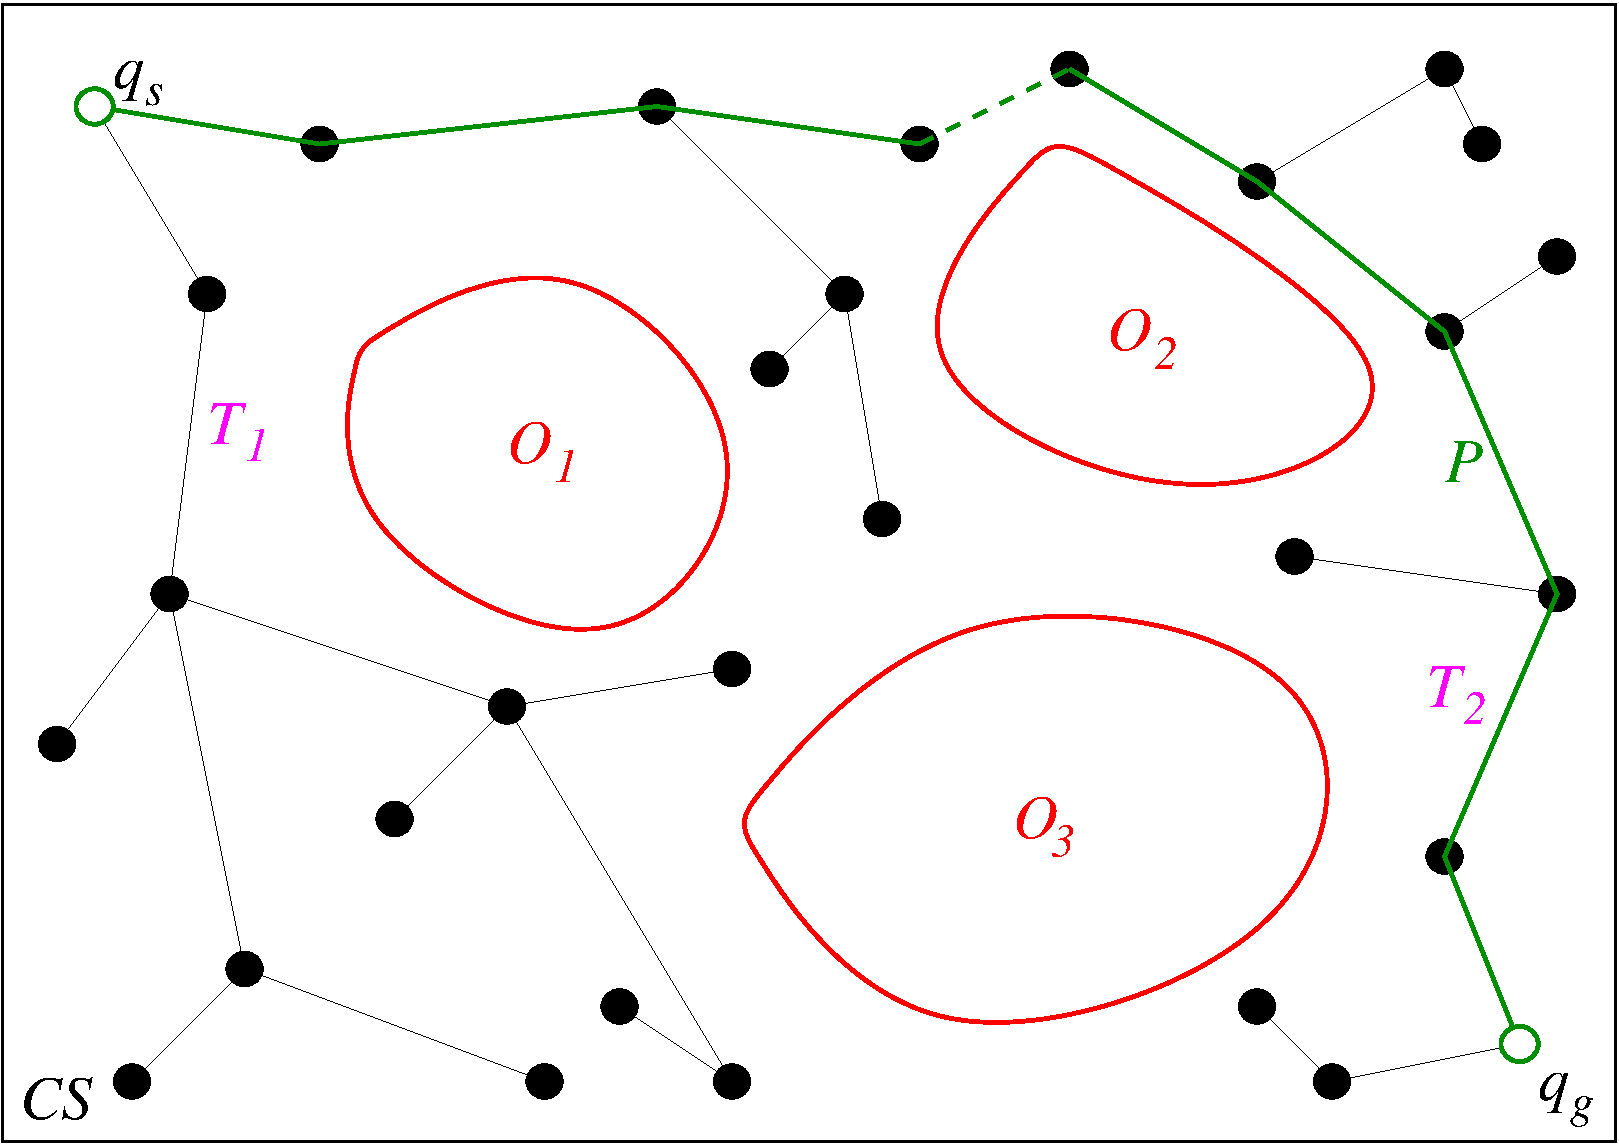
\includegraphics[width = 0.8\linewidth]
        {src/chap1-path-optimization/rrt.pdf}}
      \caption{A valid path (in green) computed with a bidirectional
        RRT planner. $q_{start}$ and $q_{goal}$ are the roots of the
        trees $\mathcal{T}_{1}$and $\mathcal{T}_{2}$ respectively. The
        algorithm keeps diffusing both trees until they can be
        connected together with an edge (in dashed green).}
      \label{fig:chap1-rrt}
\end{figure}

While not being complete (i.e.\ they cannot tell whether a solution
exists or not), sampling-based algorithms have the weaker property of
probabilistic completeness: if a solution path exists, then the
algorithm will be able to compute it with a probability of $1$ when
the number of iterations $K$ reaches infinity. In practice, these
algorithms can compute paths in complex real-life environments in a
reasonable time on regular computers and have been used to solve
problems for various systems, ranging from 6-DoF floating objects, to
50-DoF anthropomorphic systems, to 1000-DoF proteins.

\subsection{Path Optimization}
\label{subsec:chap1-path-optimization}

As shown in Figure \ref{fig:chap1-rrt}, RRT returns the shortest path
$P$ inside the graph that connects \config{s} to \config{g}. Due to
the probabilistic nature of RRT, it is clear that $P$ is not optimal
in terms of length. Path optimization methods take a valid,
i.e.\ collision-free, path as input and try to shorten it while making
sure that the output path is still valid.

\subsubsection{Greedy Optimization}

A greedy optimizer, such as the one shown in Figure
\ref{fig:chap1-optimizers}, left, uses the greedy approach to shorten
and smooth a path. First, it tries to connect directly \config{s} to
\config{g}; if the path is not collision-free, it tries to connect
\config{s} to the node preceding \config{g}, and so on until it
reaches \config{s}. This process is then restarted similarly on the
following nodes.

\subsubsection{Random Optimization}
\label{subsubsec:chap3-random-optimization}

In the case of the greedy optimizer, the nodes that are in the
optimized path are also nodes of the input path. Random Optimization
(RO) tries to bypass some nodes and keeps the rest. While this simple
method runs very fast, it does not always give the best possible
path. A different shortcut strategy can be run in a loop: at each
iteration, two random configurations are sampled on the path, and the
optimizer tries to connect \config{s} to the first, the first one to
the second one, and the second one to \config{g}. The local paths that
are still collision-free are then kept to make a shorter path, as
shown in Figure \ref{fig:chap1-optimizers}, right.

\begin{figure}
  \centering
      {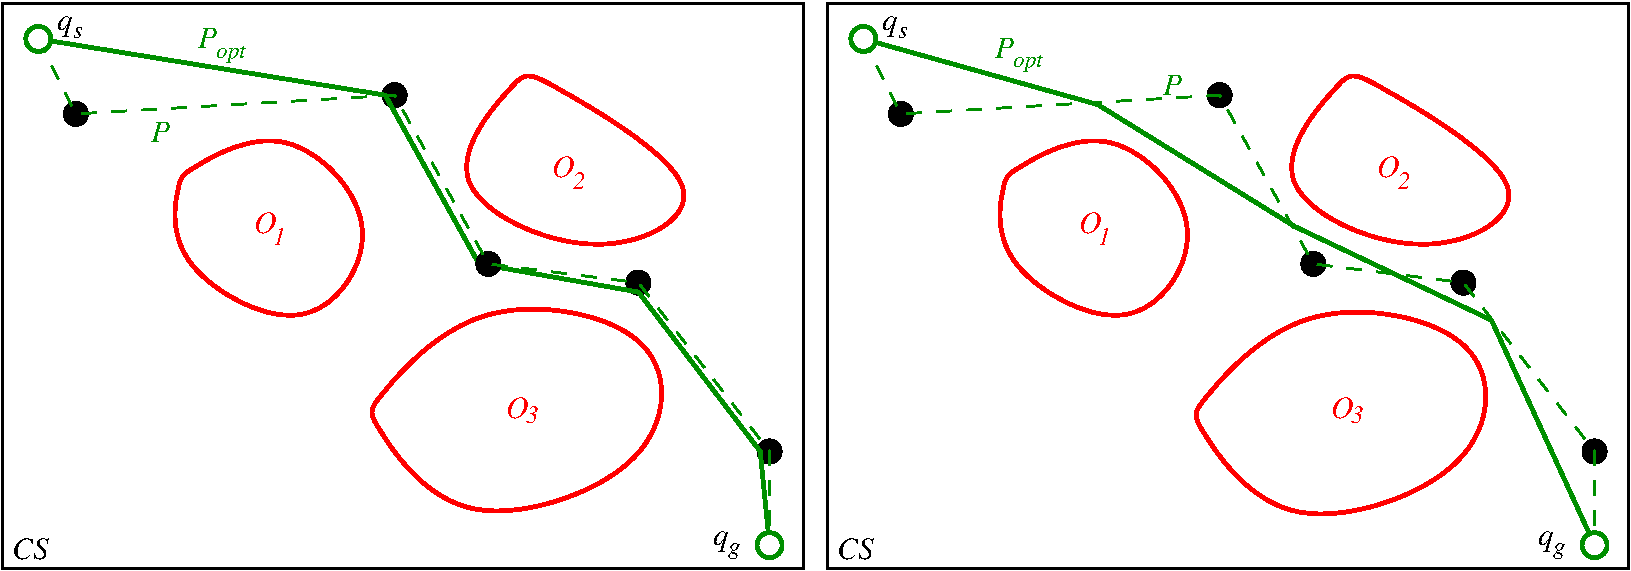
\includegraphics[width = \linewidth]
        {src/chap1-path-optimization/optimizers.pdf}}
      \caption{Left: The path $P$ (in dashed green) is optimized with
        a greedy optimizer. Right: The optimized path $P_{opt}$ (in
        continuous green) after several iterations of random
        optimization (RO).}
      \label{fig:chap1-optimizers}
\end{figure}

\section{Anthropomorphic Systems}
\label{sec:chap1-anthropomorphic-systems}

We focus in this work on humanoid robots and digital actors, which are
anthropomorphic systems. Such systems have a high number of DoF, and
are capable of accomplishing human-like tasks: locomotion (such as
walking, running and parkour), manipulation, or both. These tasks can
be accomplished thanks to the fact that anthropomorphic systems are
both underactuated and highly redundant.

In the remainder of this work, we will refer indistinguishably to
anthropomorphic systems, humanoid robots and digital actors.

\subsection{Underactuated Systems}
\label{subsec:chap1-underactuated-systems}

A robot {\robot} is usually composed of a set of rigid bodies
$($\body{i}$)_i$, $i \in 0..N_B$, and a set of joints
$($\joint{i}$)_i$, $i \in 1..N_J$, which constrain the body
positions. A rigid body has a mass, an inertia and a given
geometry. We use the kinematic tree formalism proposed in
\cite{feat08} to model a full robot: a node of the tree represents a
body of the robot, while an arc (or edge) represents a joint \joint{i}
of the robot which constrains the motion of the successor body
\body{i} with respect to its parent body \body{\lambda_{i}} (see
Figure \ref{fig:chap1-robot-kinematic-tree}). Note that in the tree
representation, each body has one and exactly one parent body, except
for the root body which has no parents; this means that additional
constraints have to be added later on in order to correctly model
robots with closed kinematic chains such as parallel robots, or
humanoid robots when they are in contact with their environment.

\begin{figure}
  \centering
      {\def\svgwidth{0.8\linewidth}
        \subimport*{src/chap1-path-optimization/}
                   {robot-kinematic-tree.pdf_tex}}
      \caption{Left: schematic view of a humanoid robot: bodies
        are connected with joints (yellow circles) which represent the
        actuators. A fictitious 6-DoF joint, or floating joint (purple
        circle), is added to move the robot in {\segroup}. Right: A
        kinematic tree view of the same robot, where bodies and joints
        are represented by nodes and edges respectively.}
      \label{fig:chap1-robot-kinematic-tree}
\end{figure}

Joints usually correspond to the actuators on the physical robot. Each
type of actuator will then have an equivalent type of joint
(prismatic, revolute, etc). A configuration \config{} of such a robot
can then be defined as the concatenation of all joint DoF values, and
the set of all configurations is called the actuated configuration
space {\actcspace}. This is however not sufficient in the particular
case of anthropomorphic systems, which rely on making and breaking
contact with their environment -- the floor for instance -- in order
to move in their workspace. Additional information in the
configuration vector is needed to model the general position of the
system, and not only its actuators. Anthropomorphic systems are
therefore said to be \emph{underactuated systems}.

We therefore introduce a 6-DoF floating joint, which we attach to the
root of the existing kinematic tree containing the actuated
joints. The successor body of the floating joint will be called the
floating base. Note that any body of the kinematic tree can be chosen
to be the floating base; in Figure
\ref{fig:chap1-robot-kinematic-tree}, the floating base is the
``waist'' of the robot. Thus, a full configuration \config{} of the
robot {\robot} is an element of the configuration space {\cspace} $=$
{\segroup} $\times$ {\actcspace}.
 
\subsection{Kinematic Redundancy}
\label{subsec:chap1-kinematic-redundancy}

\begin{figure}
  \centering
      {\def\svgwidth{0.8\linewidth}
        \subimport*{src/chap1-path-optimization/}
                   {robot-redundancy.pdf_tex}}
      \caption{Anthropomorphic systems are highly redundant
        systems. For a desired Cartesian position (in blue) of the end
        effector \body{e}, there exists more than one configuration
        \config{} that accomplish this task. Left and right: two
        possible solution configurations.}
      \label{fig:chap1-robot-redundancy}
\end{figure}

We briefly introduce here the concept of kinematic redundancy. Figure
\ref{fig:chap1-robot-redundancy} shows that for a same target
Cartesian position of the end effector \body{e}, there exists more
than one configuration of {\robot} that allows \body{e} to
reach the target. The robot {\robot} is therefore
kinematically redundant with respect to the task of reaching the
object. One could imagine assigning multiple tasks to be accomplished
at the same time, or even exploring {\cspace} while continuously
accomplishing one or more tasks. This will be discussed more
thoroughly in Chapter \ref{chap:wholebody-planning}.

\section{Walking and Balance}
\label{sec:chap1-pattern-generator}

As stated in Section \ref{subsec:chap1-underactuated-systems},
anthropomorphic systems are underactuated. This means that they have
to press some of their bodies against their environment in order to
produce a displacement. In terms of dynamics, this is equivalent to
saying that the environment exerts forces on contact surfaces of the
robot. Note, however, that not all kinds of forces can be achieved, as
the environment cannot for instance pull a body towards it in order to
retain a contact. Great care must be then given to make sure that a
planned motion is indeed achieved on a given system and
environment. The concept of \emph{balance} can be thus introduced: a
motion will be balanced, provided that there are sufficient external
forces which allow both achieving this motion and keeping the system
physical integrity. In the general case, this does not necessarily
imply that the system will not fall; a humanoid robot executing a
back-flip is technically falling in the absence of contact forces,
but, as long as it lands back safely on the ground without damaging
its bodies, sensors or actuators, this motion is deemed to be
balanced.

In this work, as we focus on the particular case of humanoid walking
on a flat floor, we can rely on results from walking system stability
analysis \cite{wieber2002} in order to verify and guarantee an
anthropomorphic system balance during a walking motion.

\subsection{Zero-Moment Point (ZMP)}
\label{subsec:chap1-zmp}

We assume here that the robot {\robot} is walking on a flat horizontal
floor, to which we associate the normal vector $\mathbf{u}$. We also
assume that the robot is always in contact with the floor using its
feet, i.e.\ that there are no jumps, and that all contacts are
non-sliding. We will call these assumptions the \emph{walking
  conditions}. {\robot}~is then subject to its weight and to contact
forces, and the total wrench of applied forces can be written as:

\begin{equation}
  \left(\begin{matrix}
    \sum_i m_i\mathbf{g}+\sum_k \mathbf{f}_{c_k} \\
    \sum_i m_i\mathbf{x}_i\times\mathbf{g}
    +\sum_k\mathbf{p}_{c_k}\times\mathbf{f}_{c_k}
  \end{matrix}\right),
\end{equation}

\noindent where $m_i$ and $\mathbf{x}_i$ are respectively the mass and
center of mass vector of rigid body \body{i}, $\mathbf{g}$ is the
gravity acceleration vector, and $\mathbf{p}_{c_k}$ and
$\mathbf{f}_{c_k}$ are respectively the position and force vectors for
contact $c_k$.

Newton's second law of motion states that the total wrench of forces
must be equal to the system dynamic wrench, denoted
$\left(\begin{matrix}\mathbf{f}\\\mathbf{n}\end{matrix}\right)$. Let
$m$ and $\mathbf{x}_G$ denote respectively the total mass of the robot
and its \emph{Center of Mass (CoM)} position. Assuming that the
walking conditions are verified, the analysis presented in
\cite{wieber2002} can be applied to guarantee that a walking motion is
\emph{dynamically balanced} if and only if the vertical projection of
the point defined by:

\begin{equation}
\label{eq:chap1-dynamic-balance}
  \frac{m\mathbf{g}\mathbf{x}_G +
    \mathbf{u}\times\mathbf{f}}{m\mathbf{g} + \mathbf{f}.\mathbf{u}}
\end{equation}

\noindent is always in the interior of the convex hull of the contact points;
the convex hull is also known as the \emph{support polygon}.

This point is called the \emph{Zero-Moment Point (ZMP)}
\cite{vukobratovic1969contribution}, where it is defined as the point
on the floor where the horizontal components of the total moment are
zero. It is also known as the \emph{Center of Pressure (CoP)}, as it
can be found by computing the barycenter of contact points weighted by
normal contact forces applied on them. We further discuss the use of
the ZMP formulation in Chapter \ref{chap:optimal-motion-planning}.

Note that in the particular case where the dynamic wrench is zero,
i.e.\ when body velocities and accelerations are zero, the point
defined in Equation \equref{eq:chap1-dynamic-balance} coincides with
the CoM. This allows us to guarantee that a quasi-static walking
motion is \emph{statically balanced} if and only if the vertical
projection of the CoM is always in the interior of the support
polygon.

\subsection{Cart-Table Model}
\label{subsec:chap1-cart-table}

The above formulation of ZMP is rather hard to control. One way to
deal with the complexity of a humanoid robot kinematic tree is to use
the so-called ``cart-table'' simplified model, where the walking robot
is modeled by a point mass at a fixed height, see Figure
\ref{fig:chap1-robot-cart-table}. The equations giving the ZMP
horizontal coordinates $(p_x,p_y)$ as functions of the CoM horizontal
coordinates $(x,y)$ in the cart-table model were presented in
\cite{kaji03}:
\begin{equation}
\label{eq:chap1-walk-zmp}
\left(
\begin{array}{c}
p_x\\ p_y
\end{array}
\right) = \displaystyle \left(
\begin{array}{c}
x - \frac{z_c}{g} \ddot{x}\\ y - \frac{z_c}{g} \ddot{y}
\end{array}
\right)
\end{equation}
\noindent where $z_c$ is the constant height of the CoM and $g$ is the gravity
constant.

\begin{figure}
  \centering
      {\def\svgwidth{0.5\linewidth}
        \subimport*{src/chap1-path-optimization/}
                   {robot-cart-table.pdf_tex}}
      \caption{Simplified model of a cart on table. The cart can move
        horizontally along one dimension on the table with a non-zero
        acceleration and represents the robot CoM. The table foot
        represents the contact surface of the robot. Note that in its
        current state, the robot is dynamically balanced, as the ZMP
        lies on the table foot. The CoM vertical projection, on the
        other hand, is outside the table foot and static balance is
        not ensured.}
      \label{fig:chap1-robot-cart-table}
\end{figure}

Based on this simplified model, a walking pattern generator is
proposed in \cite{kaji03}. Starting from a time-parameterized
footprint sequence, a reference ZMP trajectory is built such that it
connects the footprint centers and remains inside the support
polygon. The support polygon consists of one footprint in
single-support phases, and of the convex hull of two consecutive
footprints in double-support phases. A preview-control method uses
then Equation \equref{eq:chap1-walk-zmp} to derive the CoM trajectory,
see Figure \ref{fig:chap1-zmp}, and inverse-kinematics methods are
finally used to generate a whole-body dynamically balanced walking
motion of the system.

\begin{figure}
  \centering
  \definecolor{c8eff88}{RGB}{142,255,136}
\definecolor{cffc925}{RGB}{255,201,37}
\definecolor{cff5663}{RGB}{255,86,99}
\definecolor{c454545}{RGB}{69,69,69}
\definecolor{c0200d1}{RGB}{2,0,209}

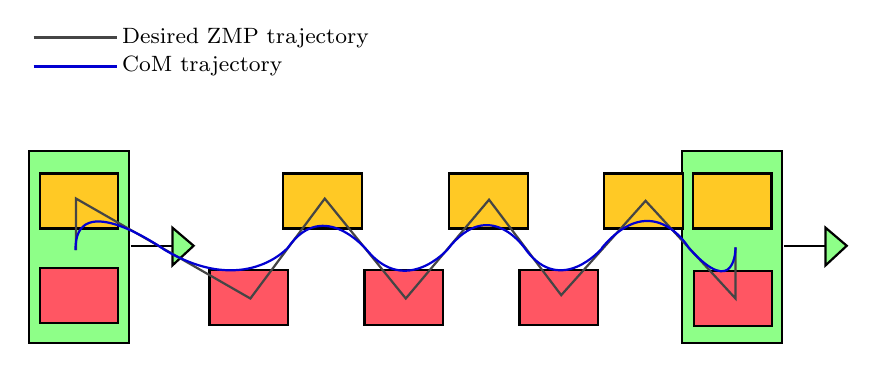
\begin{tikzpicture}[y=2.pt, x=2.pt,yscale=-1, inner sep=0pt, outer sep=0pt]
  %Start and end configurations
  \begin{scope}[cm={{0.0,1.0,-1.0,0.0,(360.33128,174.24827)}}]
    \path[draw=black,fill=c8eff88,miter limit=4.00,line width=0.800pt,rounded
      corners=0.0000cm] (47.0740,258.0597) rectangle (81.6792,276.2132);
    \path[draw=black,fill=c8eff88,line join=miter,line cap=butt,line width=0.800pt]
    (64.1273,257.7760) -- (64.1273,246.9973);
    \path[draw=black,fill=c8eff88,line join=miter,line cap=butt,line width=0.800pt]
    (64.1273,246.4300) -- (67.6730,250.2593) -- (60.8654,250.2593) -- cycle;
  \end{scope}
  \begin{scope}[cm={{0.0,1.0,-1.0,0.0,(478.33128,174.24827)}}]
    \path[draw=black,fill=c8eff88,miter limit=4.00,line width=0.800pt,rounded
      corners=0.0000cm] (47.0740,258.0597) rectangle (81.6792,276.2132);
    \path[draw=black,fill=c8eff88,line join=miter,line cap=butt,line width=0.800pt]
    (64.1273,257.7760) -- (64.1273,246.9973);
    \path[draw=black,fill=c8eff88,line join=miter,line cap=butt,line width=0.800pt]
    (64.1273,246.4300) -- (67.6730,250.2593) -- (60.8654,250.2593) -- cycle;
  \end{scope}
  %Footprints
    \path[cm={{0.0,1.0,-1.0,0.0,(0.0,0.0)}},draw=black,fill=cffc925,miter
      limit=4.00,line width=0.800pt,rounded corners=0.0000cm] (225.3161,-100.2912)
    rectangle (235.2439,-86.1087);
    \path[cm={{0.0,1.0,-1.0,0.0,(0.0,0.0)}},draw=black,fill=cffc925,miter
      limit=4.00,line width=0.800pt,rounded corners=0.0000cm] (225.3161,-144.2911)
    rectangle (235.2439,-130.1087);
    \path[cm={{0.0,1.0,-1.0,0.0,(0.0,0.0)}},draw=black,fill=cffc925,miter
      limit=4.00,line width=0.800pt,rounded corners=0.0000cm] (225.3161,-174.2911)
    rectangle (235.2439,-160.1087);
    \path[cm={{0.0,1.0,-1.0,0.0,(0.0,0.0)}},draw=black,fill=cffc925,miter
      limit=4.00,line width=0.800pt,rounded corners=0.0000cm] (225.3161,-202.2911)
    rectangle (235.2439,-188.1087);
    \path[cm={{0.0,1.0,-1.0,0.0,(0.0,0.0)}},draw=black,fill=cffc925,miter
      limit=4.00,line width=0.800pt,rounded corners=0.0000cm] (225.3161,-218.2911)
    rectangle (235.2439,-204.1087);
    \path[cm={{0.0,1.0,-1.0,0.0,(0.0,0.0)}},draw=black,fill=cff5663,miter
      limit=4.00,line width=0.800pt,rounded corners=0.0000cm] (242.4480,-100.2912)
    rectangle (252.3757,-86.1087);
    \path[cm={{0.0,1.0,-1.0,0.0,(0.0,0.0)}},draw=black,fill=cff5663,miter
      limit=4.00,line width=0.800pt,rounded corners=0.0000cm] (242.6932,-130.9444)
    rectangle (252.6209,-116.7619);
    \path[cm={{0.0,1.0,-1.0,0.0,(0.0,0.0)}},draw=black,fill=cff5663,miter
      limit=4.00,line width=0.800pt,rounded corners=0.0000cm] (242.6932,-158.9444)
    rectangle (252.6209,-144.7619);
    \path[cm={{0.0,1.0,-1.0,0.0,(0.0,0.0)}},draw=black,fill=cff5663,miter
      limit=4.00,line width=0.800pt,rounded corners=0.0000cm] (242.6932,-186.9444)
    rectangle (252.6209,-172.7619);
    \path[cm={{0.0,1.0,-1.0,0.0,(0.0,0.0)}},draw=black,fill=cff5663,miter
      limit=4.00,line width=0.800pt,rounded corners=0.0000cm] (242.8937,-218.4225)
    rectangle (252.8214,-204.2401);
  %ZMP trajectory
    \path[draw=c454545,line join=miter,line cap=butt,miter limit=4.00,line
      width=0.800pt] (92.6635,239.1801) -- (92.6635,229.8536) -- (124.1530,247.9049)
    -- (137.5913,229.8536) -- (152.2329,247.9049) -- (167.2757,230.0542) --
    (180.3127,247.3032) -- (195.5561,230.2548) -- (211.8023,247.9049) --
    (211.8023,238.6787);
  %Com trajectory
    \path[draw=c0200d1,line join=miter,line cap=butt,miter limit=4.00,line
      width=0.800pt] (92.5632,239.1801) .. controls (92.3626,227.5470) and
    (108.6088,239.0798) .. (108.6088,239.0798) .. controls (123.1502,247.7044) and
    (130.9724,238.6787) .. (130.9724,238.6787) .. controls (137.3907,229.5528) and
    (145.3132,239.2804) .. (145.3132,239.2804) .. controls (152.2329,247.5038) and
    (159.7543,239.0798) .. (159.7543,239.0798) .. controls (167.4762,229.0513) and
    (173.9948,239.1801) .. (173.9948,239.1801) .. controls (180.3127,247.5038) and
    (187.6336,238.8793) .. (187.6336,238.8793) -- (187.7338,238.6787) .. controls
    (196.9601,227.8479) and (203.3783,238.7790) .. (203.3783,238.7790) .. controls
    (211.9026,248.3061) and (211.8023,238.6787) .. (211.8023,238.6787);
  %legend
    \path[opacity=0,line join=miter,line cap=butt,line width=0.800pt]
    (85,200.7535) -- (100,200.7535)
    node[opacity=0,right] {\footnotesize Desired ZMP trajectory};
    \path[draw=c454545,line join=miter,line cap=butt,line width=0.800pt]
    (85,200.7535) -- (100,200.7535)
    node[right=2] {\footnotesize Desired ZMP trajectory};
    \path[draw=c0200d1,line join=miter,line cap=butt,line width=0.800pt]
    (85,206) -- (100,206)
    node[right=2] {\footnotesize CoM trajectory};

\end{tikzpicture}

  \caption{An illustration of the walking pattern generator: a desired
    ZMP trajectory (in grey) connects footprints. During the
    single-support phase, the ZMP stays under the support foot, and
    switches feet during the double support phase. The cart-table
    model is then used to produce the corresponding CoM trajectory (in
    blue).}
  \label{fig:chap1-zmp}
\end{figure}

\section{Humanoid Walk Planning}
\label{sec:chap1-humanoid-walk-planning}

The motion planning problem is certainly a complex one in the case of
humanoid robots, which are high-DoF redundant systems that have to
verify bipedal balance constraints. Various planning strategies can
be found in the literature.

\subsection{Footstep Planning}
\label{subsec:chap1-footstep-planning}

One possible way of addressing humanoid walk planning is by reasoning
on the footstep level. In \cite{kuff01,ches05}, humanoid footstep
planning schemes are described. Starting from an initial footstep
placement, they use an A$^{*}$ graph search \cite{hart68} to explore a
discrete set of footstep transitions. The search stops when the
neighborhood of the goal footstep placement is reached. A similar
approach \cite{garimort2011humanoid} that uses D$^*$ Lite allows fast
re-planning in the presence of dynamic obstacles. While the previous
methods are very efficient, they are not practical in environments
with narrow passages; in \cite{xia09, perr11a}, the computational cost
of footstep planning is reduced by adapting RRT planning algorithm and
efficiently exploring the discrete footstep space. In their most
recent work, \cite{perr11b, perr12} give an elegant proof of the
equivalence between the discrete footstep planning problem and a
continuous motion planning problem, which enables the use of
off-the-shelf planning algorithms such as RRT.

\subsection{Constraints-Based Motion Generation}
\label{subsec:chap1-constraints-motion-generation}

Another category relies on prioritized whole-body task planning:
kinematic redundancy is used to accomplish tasks with different orders
of priorities \cite{khatib2004wbd, saab-tro-12}. Dynamic balance and
obstacle avoidance can then be defined as unilateral constraints that
the algorithm has to verify during the whole motion. The trajectory is
then generated by specifying a set of goal tasks -- which could be a
goal configuration -- and let this set act as an attractor, in a way
similar to the simpler example shown in
\ref{subsec:chap1-deterministic algorithms}. Using such as scheme, the
work in \cite{kano09} defines a robot augmented with a sequence of
footprints and formulates the problem of locomotion planning as an
optimization problem. Such a scheme works well in the presence of
simple obstacles, but is prone to falling in local minima, failing to
find solutions for more complex environments.

\subsection{Constrained Motion Planning}
\label{subsec:chap1-constrained-motion-planning}

More recently, sampling-based motion planning algorithms were adapted
to efficiently explore a constraint submanifold of {\cspace}. In
\cite{bretl2006motion, haus10}, this strategy is used to plan on a
union of submanifolds, where each manifold is defined by a contact
limb position and static balance constraints, producing statically
balanced locomotions for hexapods and humanoid robots on uneven
terrain. Constrained motion planning will be further discussed in
Chapter \ref{chap:wholebody-planning}, where a new
dynamically-balanced locomotion planner is introduced.

\subsection{Multi-Contact Planning}
\label{subsec-chap1-multi-contact-planning}

It is interesting to note that while collision avoidance is a
requirement in motion planning, some features of the environment can
in fact be useful to solve the problem, especially in the case of
underactuated systems. In \cite{bouy12, escande2013planning}, a
multiple-contact-point stance planner looks for authorized contact
surfaces in order to help the robot reach its goal. The contact points
do not have to be coplanar, and the planner produces a sequence of
statically balanced postures for a humanoid robot which can press his
feet and hands against objects in the environment. A~heuristic method
is used to direct the search towards the goal, so this planner does
not offer a completeness property. Once the contact stance sequence is
obtained, motion generation tools can be used to generate
statically balanced or dynamically balanced locomotion trajectories.

\subsection{Decoupled Planning}
\label{subsec:chap1-bounding-box}

Finally, another strategy consists in dividing a high-dimensional
problem into smaller problems and solving them successively
\cite{zhan09}. The idea of dividing the problem into a two-stage
scheme is described in \cite{yosh08}: A 36-DoF humanoid robot is
reduced to a 3-DoF bounding box. Using the robot simplified model, the
PRM algorithm solves the path planning problem and generates a valid
path for the bounding box. A geometric decomposition of the path
places footsteps on it, and the walk pattern generator described in
Section \ref{sec:chap1-pattern-generator} finally produces the
whole-body trajectory for the robot. In \cite{moul10}, this two-stage
approach is also used; numerical optimization of the bounding box path
produces a time-optimal trajectory that is constrained by foot speed
and distance to obstacles. Optimization techniques will be discussed
in details in Chapter \ref{chap:optimal-motion-planning}, where we
describe an optimal motion planning framework.

\subsection{Holonomic vs Nonholonomic Walking Motion}
\label{subsec:chap1-holonomic}

An important notion on humanoid walk planning is the one of holonomic
motion.
A \emph{holonomic} \emph{constraint} is given by:
\begin{eqnarray} C(\mathbf{q}) & = & 0,
  \label{eq:chap1-holonomic_constraint}
\end{eqnarray}
with \config{} the configuration vector. When a constraint of the form
\begin{eqnarray}
  C(\mathbf{q,}\overset{.}{\mathbf{q}}) & = & 0,
\end{eqnarray}
with $\mathbf{\overset{.}{\mathbf{q}}=}\frac{d\mathbf{q}}{dt}$, cannot
be integrated into a form similar to \equref{eq:chap1-holonomic_constraint},
this constraint is called \emph{nonholonomic}.

In practice, a nonholonomic constraint implies that a system velocity
vector cannot take an arbitrary direction. For instance, you cannot
drive a car sideways (this makes life harder for us when parking), and
therefore it has a nonholonomic constraint. On the other hand, a
spherical ball can roll in any direction, which means it has a
holonomic constraint.

So is there a particular constraint that governs human gait? Studies,
like the one described in \cite{momb10}, established a model that
presents trajectory planning as an optimization problem of a cost
function. Basically, it is shown that for small distances and small
orientation variations between the start and goal configurations,
humanoid motion obeys a holonomic constraint, and sidestepping is
allowed. However, for greater distances and orientation variations, a
nonholonomic constraint rules human gait, and sidestepping is
forbidden, i.e.\ the human direction is always tangent to its path.
But one should note that this model is only applicable in the case of
the absence of any obstacles, and it is clear that in the presence of
narrow passages, a human would be forced to adopt holonomic motion in
order to walk sideways.

The path planning scheme in \cite{yosh08} is designed to this end; a
PRM algorithm first builds a roadmap with Dubins curves \cite{dubi57},
but such curves impose a nonholonomic constraint and narrow passages
cannot be crossed. The roadmap is therefore enriched with linear local
paths. As a result, this planning scheme generates motions such that
the robot remains tangent to its path most of the time and uses
sidestepping only in narrow passages.

\section{Contribution: Regular Sampling Optimization}
\label{sec:chap1-contribution}

The work of \cite{moul10} provides a sound way for generating nice
walking trajectories, using numerical optimization to minimize the
robot walking time along the path while enforcing velocity and
obstacle distance constraints. However, after having tried this
approach, we came to the conclusion that it was too computationally
expensive given the simple nature of the robot model, with
optimizations taking several minutes even for simple environments.

While using the same two-stage approach of \cite{yosh08}, a simpler
heuristic method that generates near time-optimal humanoid
trajectories is proposed. First the PRM algorithm and the Dubins local
paths are replaced with an RRT-Connect algorithm and linear local
paths. The path is then optimized by locally reorienting the robot
bounding box on a discrete set of configurations. Our heuristic gives
priority to nonholonomic motion; holonomic motion is used only to pass
in narrow passages or avoid nearby obstacles, thus generating short
walking trajectories.

The following section presents this method and explains how it is
integrated in the motion planning scheme. Examples of different
scenarios, including a real one with the HRP-2 platform, are shown in
\autoref{sec:chap1-examples}.

\section{Regular Sampling Optimization}
\label{sec:chap1-regular-sampling-optim}

\begin{figure}
  \centering
      {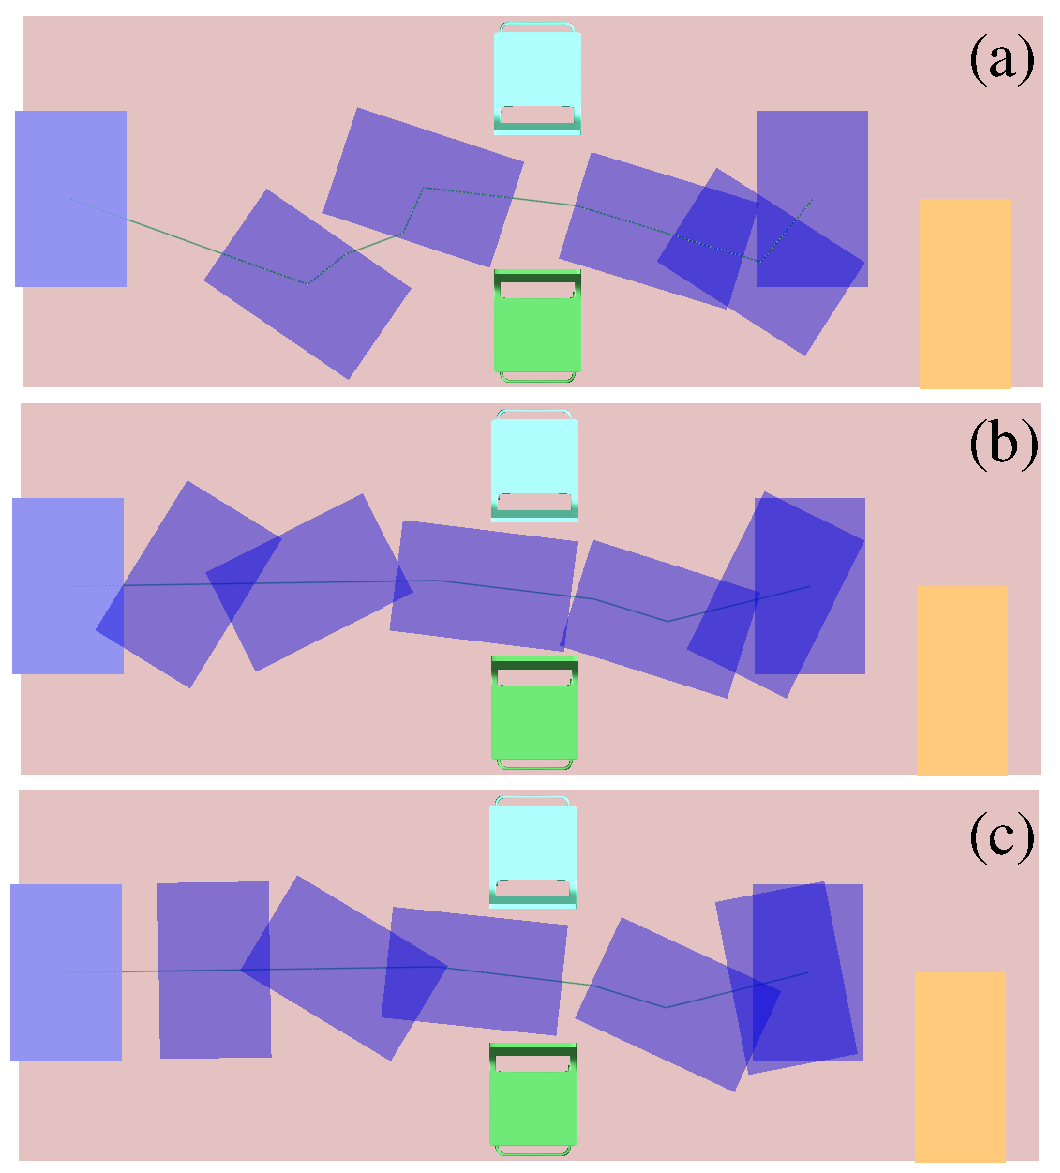
\includegraphics[width = 0.8\linewidth]
        {src/chap1-path-optimization/bb-plan-optim.pdf}}
      \caption{Top view: (a) RRT-Connect path for the bounding box
        passing between two chairs. (b) Optimized bounding box path by
        random optimization (RO). (c) Optimized bounding box after
        adding regular sampling optimization (RSO) .}
      \label{fig:chap1-bb-plan-optim}
\end{figure}

Assuming full knowledge of the environment, the RRT algorithm produces
\linebreak a collision-free piecewise linear path $P_{RRT}$ for the
robot bounding box (in offline mode), i.e.\ the path consists of the
concatenation of linear local paths $LP_{RRT}$.

Due to the probabilistic nature of RRT, $P_{RRT}$ may not be optimal
in terms of length, and a preliminary random shortcut optimization
(RO) can be run in order to shorten it (See
\autoref{fig:chap1-bb-plan-optim}). Though the optimized path $P$ is
collision-free, the bounding box orientation is such that it could
lead to a trajectory which is not time-optimal. For instance, the
humanoid robot could spend a long time walking sideways or backwards
over a long distance in an open space. An additional optimization
stage is introduced to address this issue in the next section.

\subsection{Bounding Box Path Optimization}
Note that each configuration \config{} can be written as $\mathbf{q} =
(\mathbf{X},~\theta)$, where $\mathbf{X} = (x,~y)$ describes the
bounding box position in the horizontal plane, and $\theta$ gives its
orientation.  The optimizer reorients the bounding box along $P$ by
changing $\theta$ while retaining the value of $\mathbf{X}$.

For this purpose, an A$^{*}$ search algorithm is executed. First, $P$
is regularly sampled. Using a discrete set of admissible orientations
for each sample configuration, a cost function and a heuristic
estimation function, the bounding box orientation is then modified
along $P$. An optimized path $P_{opt}$ is created and leads to a
trajectory which is time-optimal with the respect to the expanded
graph.

\subsubsection{Preliminary Notations}
After running RO on the piecewise linear path $P_{RRT}$, the
path $P$ is also piecewise linear, and its first and last
configurations are denoted by $\mathbf{q}_s$ and $\mathbf{q}_g$.

Let $d_{sample} \in \mathbb{R}^+\setminus\{0\}$ be a sampling
distance. Sampling $P$ with a distance $d_{sample}$ means dividing
each local path $LP_j$ of $P$ into smaller local paths of length
$d_{sample}$; each new local path end is then a sample
configuration. Note that the last interval on each local path $LP_j$
can have a length smaller than $d_{sample}$. The $n^{th}$ sample
configuration of $P$ in its initial state can be obtained by indexing
new local path ends starting from $\mathbf{q}_s$, and is denoted
$\mathbf{q}_n^{init}$.

\begin{figure}
  \centering
      {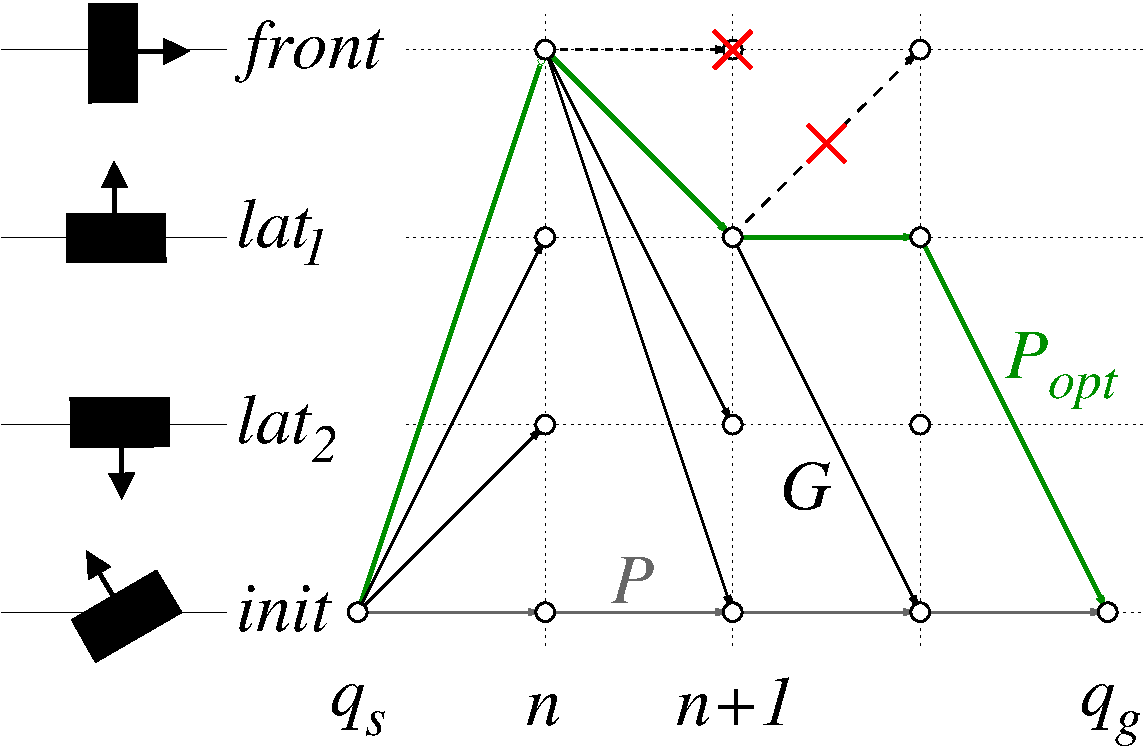
\includegraphics[width = 0.75\linewidth]
        {src/chap1-path-optimization/A-star.pdf}}
      \caption{Each initial sample configuration can be rotated and be
        in one of four states. Starting from $\mathbf{q}_s$, the
        A$^{*}$ search algorithm searches the graph $G$ that contains
        only valid nodes and arcs to produce an optimized path
        $P_{opt}$.}
      \label{fig:chap1-A-star}
\end{figure}

The admissible orientation states need to be defined. We aim to make a
humanoid robot reach its goal as soon as possible. Since the robot is
faster while walking straight than side-stepping, we attempt to change
the orientation of each initial sample configuration
$\mathbf{q}_n^{init}$ such that the bounding box is tangent to the
local path, and we introduce a new configuration denoted
$\mathbf{q}_n^{front}$. To take into account the fact that there may
be obstacles that forbid a frontal orientation, we also create
$\mathbf{q}_n^{lat_1}$ and $\mathbf{q}_n^{lat_2}$ that are rotated by
$\frac{\pi}{2}$ and $-\frac{\pi}{2}$ relative to the path tangent, see
\autoref{fig:chap1-A-star}. One particular case is local path end
configurations: the mean direction of the two adjacent local paths is
considered to define frontal and lateral configurations. This is done
to ensure a smooth transition between two local paths.

A sample configuration whose orientation is unknown will be denoted by
$\mathbf{q}_n^{state}$. It can have any orientation state of the set
$\{init,~front,~lat_1,~lat_2\}$ except for $\mathbf{q}_s$ and
$\mathbf{q}_g$ which remain in their initial state.  Ideally, the
algorithm should be able (as long as there are no obstacles) to put
each sample configuration in the frontal state, create a new path
$P_{opt}$ and generate a time-optimal trajectory for the robot.

An A$^{*}$ search is run to achieve this goal; the algorithm functions are
described in the following section.

\subsubsection{A$^{*}$ Function Definition}
\label{sec:chap1-A-star}
An A$^{*}$ search algorithm can find an optimal path in a graph as
long as the latter and an evaluation function are correctly
defined. Starting from $\mathbf{q}_s$, A$^{*}$ expands in each
iteration the admissible transitions from one sample to the next one
in the graph and evaluates, using the evaluation function, a lower
bound of the cost-to-go from each state to the goal state, see
\autoref{fig:chap1-A-star}.

A graph $G$ is defined to be a set of nodes and arcs. A valid node
$\mathbf{q}_n^{state_n}$ is defined to be a configuration with no
collisions, and a valid arc
$\mathbf{q}_n^{state_n}\mathbf{q}_{n+1}^{state_{n+1}}$ is a
collision-free local path. The whole graph $G$ could be built before
running A$^{*}$ by testing all nodes and arcs and making sure they are
collision-free. But collision tests are slow, and A$^{*}$ uses a
heuristic estimation function to avoid going through all nodes. An
empty graph $G$ is thus initialized and nodes and arcs are built only
when necessary. A successor operator needs to be defined for this
purpose.

\begin{figure}
  \centering
      {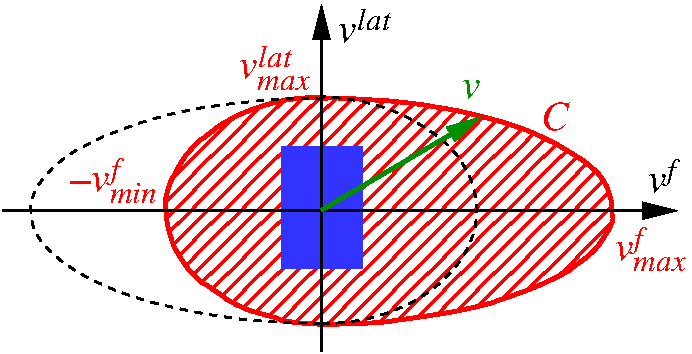
\includegraphics[width = 0.75\linewidth]
        {src/chap1-path-optimization/elliptic-constraint.pdf}}
      \caption{The rectangular bounding box speed vector $v$ is
        bounded inside the hashed area defined by the speed constraint
        $C$. The area is bounded by the union of two half-ellipsoids.}
      \label{fig:chap1-elliptic-constraint}
\end{figure}

\paragraph{The Successor operator $\Gamma(\mathbf{q}_n^{state_n})$:}
Its value for any node $\mathbf{q}_n^{state_n}$ is \linebreak a set
$\{(\mathbf{q}_{n+1}^{state_{n+1}},~c_{n,n+1})\}$, where
$\mathbf{q}_{n+1}^{state_{n+1}}$ denotes a successor node, and
$c_{n,n+1}$ is the cost of going from $\mathbf{q}_n^{state_n}$ to
$\mathbf{q}_{n+1}^{state_{n+1}}$. The cost $c_{n,n+1}$ is defined to
be the distance
$D(\mathbf{q}_n^{state_n},~\mathbf{q}_{n+1}^{state_{n+1}})$ between
two nodes of $G$; it computes the walk time from
$\mathbf{q}_n^{state_n}$ to $\mathbf{q}_{n+1}^{state_{n+1}}$. The
speed constraint $C$ is defined as:
\begin{equation}
C = \left\{
\begin{array}{l l l}
  (\frac{v^{f}}{v_{max}^{f}})^2 +
  (\frac{v^{lat}}{v_{max}^{lat}})^2 - 1
  \quad \text{if } v^f >= 0 \\

  \\

  (\frac{v^{f}}{v_{min}^{f}})^2 +
  (\frac{v^{lat}}{v_{max}^{lat}})^2 - 1
  \quad \text{if } v^f < 0
\end{array} \right.
\end{equation}
\noindent where $v^{f}$ and $v^{lat}$ are respectively the frontal and lateral
speed, and $v_{min}^f$, $v_{max}^{f}$ and $v_{max}^{lat}$ their
minimum and maximum values (See
\autoref{fig:chap1-elliptic-constraint}). $D(\mathbf{q}_n^{state_n},
~\mathbf{q}_{n+1}^{state_{n+1}})$ can be then computed by integrating
this speed constraint along the linear path connecting
$\mathbf{q}_n^{state_n}$ to $\mathbf{q}_{n+1}^{state_{n+1}}$.

Having expressed the successor operator, which allows the optimizer to
choose which node to expand at each iteration, the A$^{*}$ evaluation
function can be defined.

\paragraph{The Evaluation Function $\hat{f}(\mathbf{q}_n^{state})$:}
It is the estimated cost of an optimal path going through
$\mathbf{q}_n^{state}$ from $\mathbf{q}_s$ to $\mathbf{q}_g$ and can be written as:
\begin{equation}
  \hat{f}(\mathbf{q}_n^{state}) = \hat{g}(\mathbf{q}_n^{state}) +
  \hat{h}(\mathbf{q}_n^{state})
\end{equation}
\noindent where $\hat{g}(\mathbf{q}_n^{state})$ is the estimated cost of the
optimal path from $\mathbf{q}_s$ to $\mathbf{q}_n^{state}$ and
$\hat{h}(\mathbf{q}_n^{state})$ is a heuristic function giving the
estimated cost of the optimal path from $\mathbf{q}_n^{state}$ to
$\mathbf{q}_g$.

$\hat{h}(\mathbf{q})$ must verify $\hat{h}(\mathbf{q}) \leq
h(\mathbf{q})$ for any $\mathbf{q}$ to ensure that the algorithm is
admissible, i.e.\ that the path from $\mathbf{q}_s$ to $\mathbf{q}_g$
is optimal. Since the robot is fastest while walking straight forward
in the absence of obstacles, $\hat{h}(\mathbf{q}_n^{state})$ is
defined as:
\begin{equation}
  \begin{split}
  \hat{h}(\mathbf{q}_n^{state}) &= D(\mathbf{q}_n^{state},~\mathbf{q}_{n+1}^{front}) \\
  &+ \sum_{k=1}^{N_{sample}-n-2} D(\mathbf{q}_{n+k}^{front},~\mathbf{q}_{n+k+1}^{front}) \\
  &+ D(\mathbf{q}_{n+1}^{front},~\mathbf{q}_g)
  \end{split}
\end{equation}
\noindent where $N_{sample}$ is the total number of initial sample
configurations in $P$ including $\mathbf{q}_s$ and
$\mathbf{q}_g$. $\hat{h}(\mathbf{q}_n^{state})$ thus sums the cost of
walking along $P$ while staying tangential to the path with the start
and end transition costs from $\mathbf{q}_n^{state}$ and to
$\mathbf{q}_g$.

Now that the A$^{*}$ functions are fully defined, a search algorithm
can be run to compute an optimal path $P_{opt}$ by changing the
orientation of each sample node. Algorithm \ref{algo:chap1-rso}
describes the \emph{Regular Sampling Optimization (RSO)} method, and
an example is shown in \autoref{fig:chap1-hash-direct-path}.

\begin{algorithm}
\caption{\texttt{RSO}($P$, $d_{sample}$)}
\label{algo:chap1-rso}
\begin{algorithmic}
  \STATE {\color{red} // Closed set}
  \STATE $\mathcal{C} \leftarrow \emptyset$
  \STATE {\color{red} // Open set}
  \STATE $\mathcal{O} \leftarrow \{(\mathbf{q}_s,\hat{f}(\mathbf{q}_s))\}$
  \STATE $\mathbf{q}_n^{state_n} \leftarrow \mathbf{q}_s$
  \WHILE{$\mathbf{q}_n^{state_n} \neq \mathbf{q}_g$}
  \STATE $\mathcal{C} \leftarrow \mathcal{C}\cup\{(\mathbf{q}_n^{state_n},\hat{f}(\mathbf{q}_n^{state_n}))\}$
  \STATE {\color{red} // Expand node}
  \STATE $\mathcal{E}_{n+1} \leftarrow \{(\mathbf{q}_{n+1}^{state_{n+1}},~c_{n,n+1})\} \leftarrow \text{Expand}(\mathbf{q}_n^{state_n}, P, d_{sample})$
  \FOR{$\mathbf{q}_{n+1}^{state_{n+1}} \in \mathcal{E}_{n+1}$}
  \STATE {\color{red} // Mark as ``open'' each successor not already marked ``closed''}
  \IF{$(\mathbf{q}_{n+1}^{state_{n+1}},\hat{f}) \notin \mathcal{C}$}
  \STATE $\mathcal{O} \leftarrow \mathcal{O}\cup\{(\mathbf{q}_{n+1}^{state_{n+1}},\hat{f}(\mathbf{q}_{n+1}^{state_{n+1}})\}$
  \ELSE
  \STATE {\color{red} // Remark as open each closed successor for which evaluation function is now smaller than stored value}
  \IF{$\hat{f}(\mathbf{q}_{n+1}^{state_{n+1}}) < \hat{f}$}
  \STATE $\mathcal{O} \leftarrow \mathcal{O}\cup\{(\mathbf{q}_{n+1}^{state_{n+1}},\hat{f}(\mathbf{q}_{n+1}^{state_{n+1}})\}$
  \ENDIF
  \ENDIF
  \ENDFOR
  \STATE {\color{red} // Select open node whose value evaluation function value is the smallest}
  \STATE $\mathbf{q}_n^{state_n} \leftarrow
  \text{arg}\min_{\mathbf{q}\in\mathcal{O}}\hat{f}(\mathbf{q})$
  \ENDWHILE
  \STATE $\mathcal{C} \leftarrow \mathcal{C}\cup\{(\mathbf{q}_g,0)\}$
  \STATE {\color{red} // Return closed set which makes up optimized path.}
  \RETURN $\mathcal{C}$
\end{algorithmic}
\end{algorithm}

\begin{figure}
  \centering
      {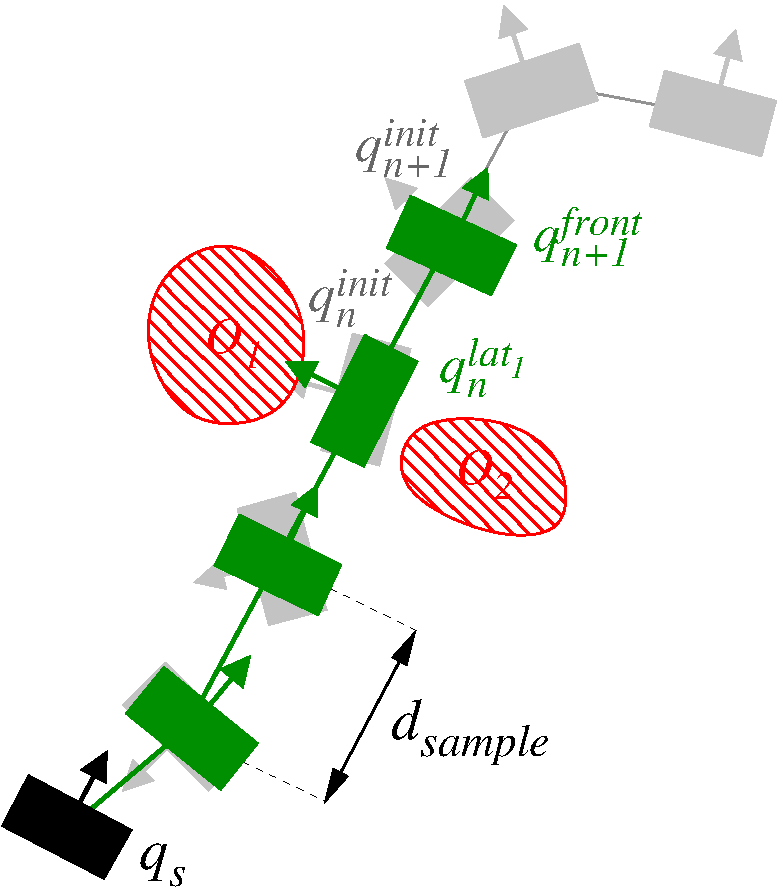
\includegraphics[width = 0.6\linewidth]
        {src/chap1-path-optimization/hash-direct-path.pdf}}
      \caption{Local paths are regularly sampled (light grey) and each
        sample configuration is reoriented (dark) while considering
        obstacles $O_1$ and $O_2$.}
      \label{fig:chap1-hash-direct-path}
\end{figure}

\subsection{Motion Generation for a Humanoid Robot}

A collision-free path $P$ for the 3-DoF bounding box can be found
using RRT-Connect and RO. The regular sampling optimization (RSO),
which is the subject of this work, is then applied on the path and
produces a path $P_{opt}$ that gives priority to nonholonomic motion.

Once the bounding box trajectory is computed, the robot has to walk
along it. A footstep sequence is thus generated along $P_{opt}$ by
geometric decomposition of the path, and the pattern generator cited
in Section \ref{sec:chap1-humanoid-walk-planning} then produces the
robot whole-body trajectory.

\section{Examples}
\label{sec:chap1-examples}

\begin{table}
\centering
\begin{tabular}{c|c|c|c|c|c|}
  \cline{2-6}
  & RRT-Connect & RO & RSO & Robot Trajectory & Total\\
  \hline
  \multicolumn{1}{|c|}{Chairs} & $3.97$ & $1.89$ & $2.14$ & $66.1$ & $74.1$\\
  \hline
  \multicolumn{1}{|c|}{Boxes} & $0.0917$ & $2.50$ & $0.238$ & $65.7$ & $68.6$\\
  \hline
  \multicolumn{1}{|c|}{Apartment} & $1.21$ & $2.43$ & $2.41$ & $223$ & $229$ \\
  \hline
\end{tabular}
\caption{Computational time, in seconds, of each planning stage for
  the presented scenarios.}
\label{tab:chap1-computation-time}
\end{table}

\begin{table}
\centering
\begin{tabular}{c|c|c|}
  \cline{2-3}
  & RO & RO+RSO \\
  \hline
  \multicolumn{1}{|c|}{Chairs} & $40$ & $35$ \\
  \hline
  \multicolumn{1}{|c|}{Boxes} & $66$ & $57$ \\
  \hline
  \multicolumn{1}{|c|}{Apartment} & $200$ & $120$ \\
  \hline
\end{tabular}
\caption{Humanoid robot walk time, in seconds, for the presented
  scenarios using RO alone and a RO-RSO combination.}
\label{tab:chap1-walk-time}
\end{table}

\begin{figure}
  \centering
      {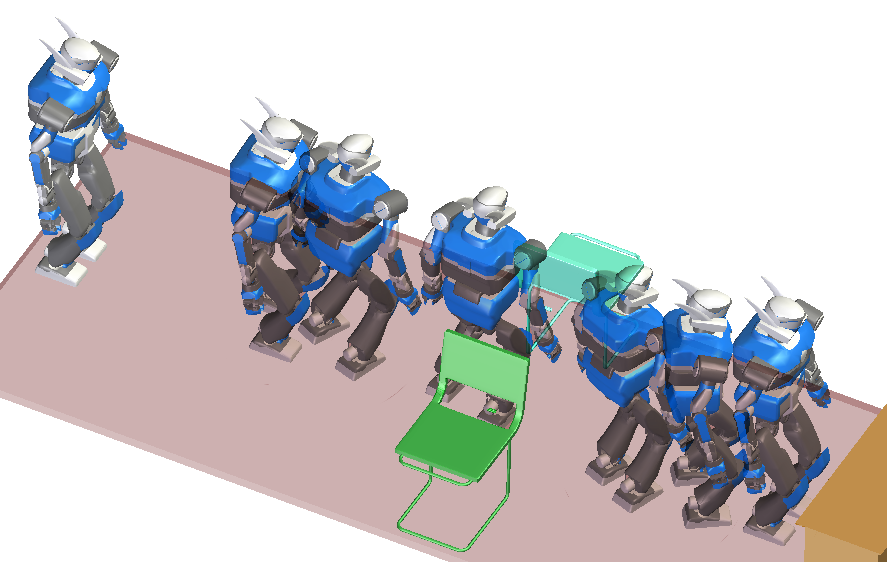
\includegraphics[width = 0.8\linewidth]
        {src/chap1-path-optimization/chairs-hash-optim-perspective-hrp2.png}}
      \caption{Perspective view of the simulated HRP-2 trajectory on
        the final optimized path passing between two chairs.}
      \label{fig:chap1-chairs-hash-optim-perspective-hrp2}
\end{figure}

This section presents experimental results of the path optimizer after
it has been inserted in the previously described walk planning
scheme. Distance parameters $v_{max}^f$, $v_{max}^{lat}$, $v_{min}^f$
are set to 0.5, 0.1, and 0.25 $m.s^{-1}$ respectively. Note that these
parameters play a key role in giving priority to forward walking with
respect to lateral and backwards walking. Indeed kinematic constraints
are usually such that it is very hard to achieve fast lateral
walking. Also sensors, such as the cameras facing the forward
direction, can require preferring forward walking to backward walking.

Since the A$^{*}$ search only takes place over the graph of
discretized configurations of the input path, it is important to
choose a proper value of the sampling interval $d_{sample}$. If the
value is too small, the search space will be much bigger, possibly
leading to better trajectories, but leading to an explosion of the
A$^{*}$ search time. If the value is too high, the A$^{*}$ search will
be very fast in the small trajectory space, but we risk missing some
optimizations on the trajectory. We found that setting $d_{sample}$ to
be equal to $\frac{h}{6}$, where $h$ is the humanoid height, provided
a good tradeoff between computation time and trajectory quality;
$d_{sample}$ gives then a broad approximation of the nominal human
step length.

Tests are performed on a 2.13 GHz Intel Core 2 Duo PC with 2 GB RAM.
Simulations of the humanoid robot HRP-2 are run in three scenarios.
The first one is a small environment where HRP-2 has to pass between
two chairs. The second environment is uncluttered with few obstacles
lying around, while the last one is a bigger apartment environment
where the robot has to move from one room to another while passing
through doors. The chairs scenario motion is also replayed on the real
humanoid robot HRP-2 \cite{kane04}, see Figure
\ref{fig:chap1-hrp2-chairs}.

\begin{figure}
  \centering{
    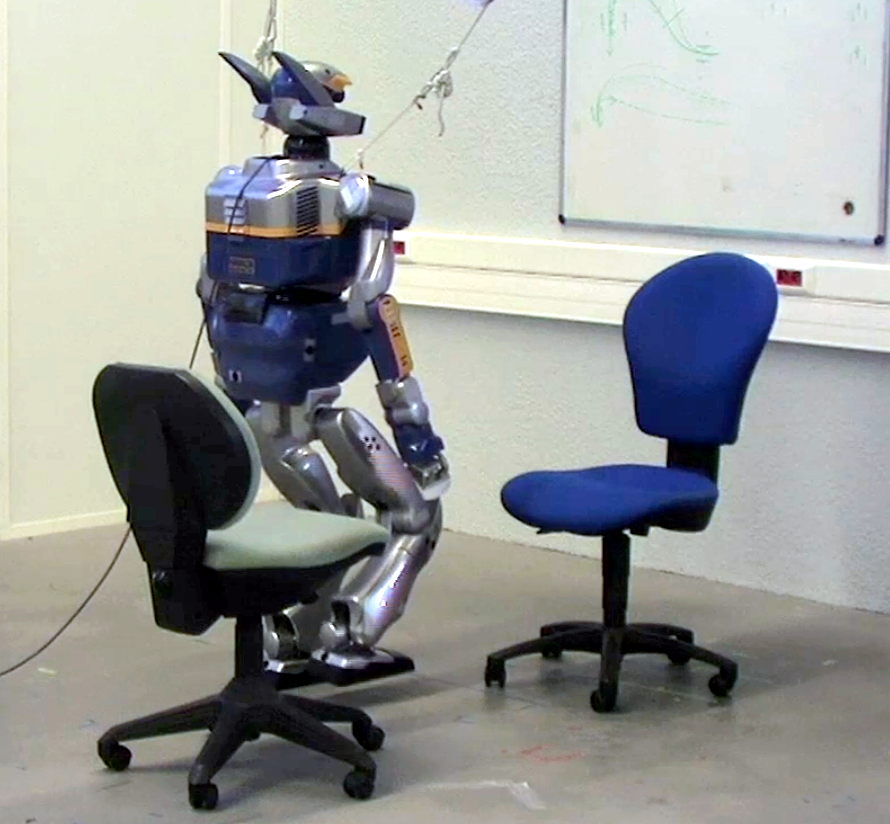
\includegraphics[width = 0.7\linewidth]
                    {src/chap1-path-optimization/hrp2-chairs.png}}
  \caption{Humanoid Robot HRP-2 uses holonomic motion, or
    side-stepping, to pass between two chairs.}
  \label{fig:chap1-hrp2-chairs}
\end{figure}

Table \ref{tab:chap1-computation-time} shows computation times for
each stage of the planning scheme: RRT-Connect, RO, RSO, and the
whole-body robot trajectory generation. In order to show the optimizer
contribution, robot walk times are also measured by creating a
trajectory directly after RO, and comparing it with a trajectory where
the RSO was added, see Table \ref{tab:chap1-walk-time}.

\subsection{``Chairs'' Scenario}
\label{subsec:chap1-chairs}

Figure \ref{fig:chap1-bb-plan-optim} shows the bounding box RRT path
and the RO path for the chairs scenario. It is obvious that RO creates
a shorter path. However, the bounding box starts rotating from the
beginning of the path even though both chairs are still far. This
causes the robot trajectory to not be time-optimal since walking
sideways takes a longer time than walking straight.

\begin{figure}
  \centering
      {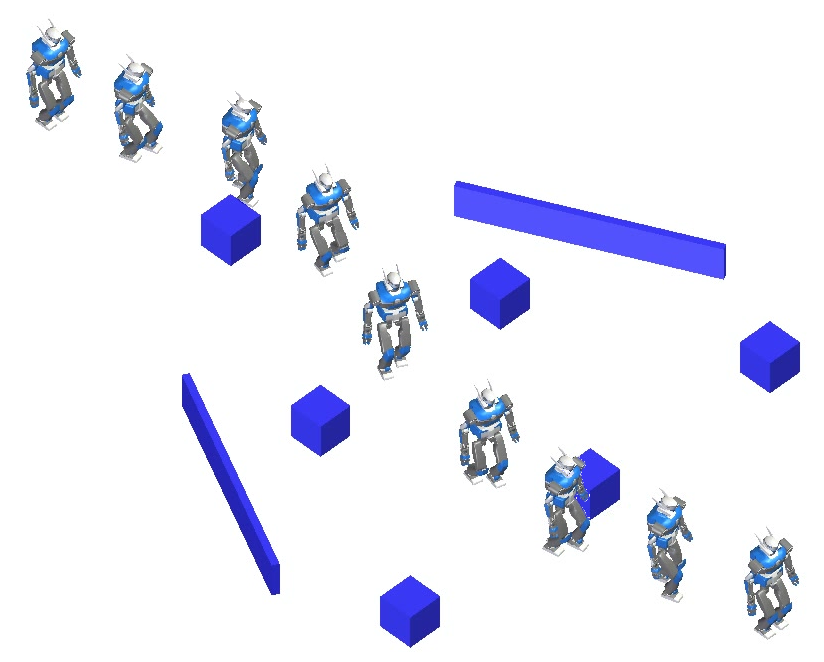
\includegraphics[width = 0.8\linewidth]
        {src/chap1-path-optimization/galton-hash-optim-perspective-hrp2.png}}
      \caption{Perspective view of HRP-2 optimized trajectory in the
        boxes scenario.}
      \label{fig:chap1-galton-hash-optim-perspective-hrp2}
\end{figure}

However, after applying RSO, it is clear that the bounding box stays
oriented towards the front and rotates only when it reaches the
chairs. \autoref{fig:chap1-chairs-hash-optim-perspective-hrp2} and
\autoref{tab:chap1-walk-time} show that the walk time is 12\% shorter
and the final trajectory for HRP-2 is more realistic. Note that the
RSO takes 2,144 ms to be executed on the chairs path, which is less
than 3\% of the total computation time.

\subsection{``Boxes'' Scenario}
Here, an uncluttered environment is considered, and it can be seen
that RRT-Connect and RSO computation times are very low compared to
other environments. This can be explained by the fact that a tree
connecting start and goal configurations is easier to find, and that
the frontal orientation state is valid for all considered samples on
the path, see Figure \ref{fig:chap1-galton-hash-optim-perspective-hrp2}.

\subsection{``Apartment'' Scenario}
The planning scheme is finally applied in the apartment scenario. In
\autoref{fig:chap1-apartment-hash-optim-perspective-hrp2}, it is
evident that HRP-2 walks facing forward through the doors. As with
previous scenarios, the trajectory is more realistic than a trajectory
where RSO is not used. The added computation time for RSO is 2,412 ms,
which is insignificant compared to the 228 seconds which are required
by the whole planning scheme.

Additionally, since the environment is significantly larger and more
constrained than the previous ones, the walk time difference is more
striking: \autoref{tab:chap1-walk-time} shows that it takes the robot
40\% less time to cross the apartment when an RO-RSO combination is
used.

\begin{figure}
  \centering
      {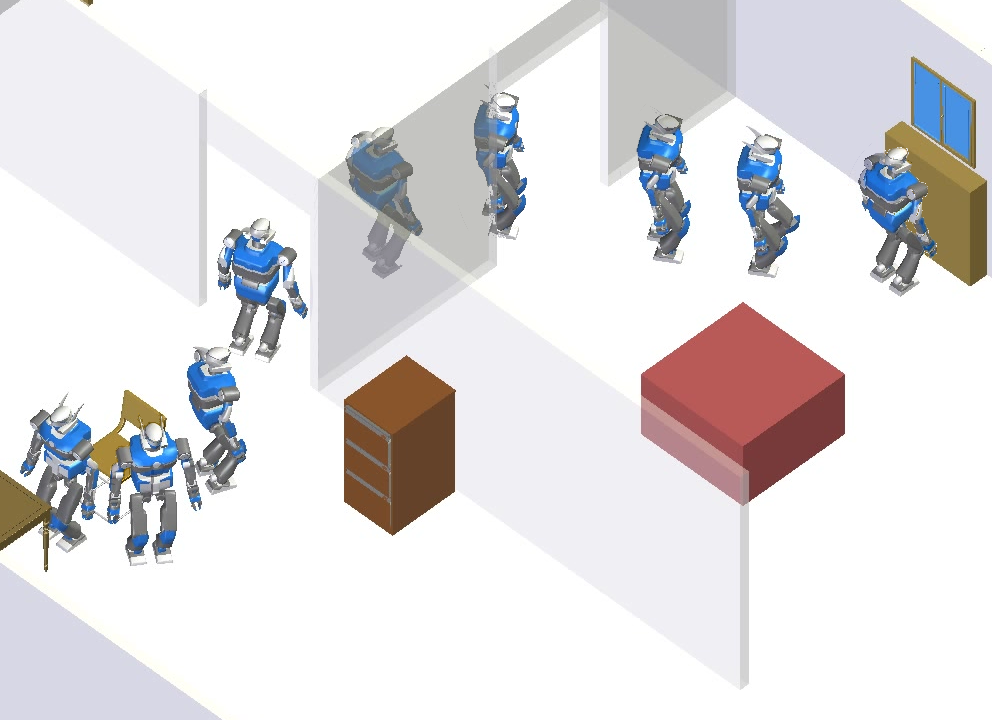
\includegraphics[width = 0.8\linewidth]
        {src/chap1-path-optimization/apartment-hash-optim-perspective-hrp2.png}}
      \caption{Perspective view of HRP-2 optimized trajectory in the
        apartment scenario.}
      \label{fig:chap1-apartment-hash-optim-perspective-hrp2}
\end{figure}

\section{Conclusion}
In this chapter, a novel simple optimization method is
presented for humanoid walk planning that relies on a decoupling
between trajectory and robot orientations. It uses an A$^{*}$ search that
takes as input a path for the robot bounding box, and produces a path
where a discrete set of configurations have been reoriented to generate
a realistic time-optimal walk trajectory. Results show that new
trajectories are more satisfactory while the added computation time is
insignificant compared to the whole planning time.

Achieving humanoid walk planning on flat surfaces using the bounding
box approach is both simple and efficient; it allows using
off-the-shelf sampling-based planners to efficiently explore the
configurations space, thus removing the need to take into account
additional kinematic and balance constraints when planning for the
whole articulated robot. But it has one major drawback: in order to
have a sound framework which always produces collision-free walking
trajectories, the bounding box must contain all the robot geometries
and take into account the robot swaying motion during walking. Thus,
it is a rather conservative method which cannot be used for
manipulation tasks, and which might not even succeed in finding
collision-free walk trajectories in cluttered environments. If we go
back to the chairs example in Section \ref{subsec:chap1-chairs}, we
can show that the lateral walking motion could have been avoided if
the HRP-2 had lifted its arms over the two chairs. Beside leading to
an even faster motion, walking forward could be necessary if vision
systems were needed to achieve robot localization and/or environment
mapping.

In the next chapter, we introduce a sound whole-body motion planning
algorithm that allows planning collision-free walking trajectories for
the fully articulated humanoid robot, hence releasing it from its
bounding box constraint and increasing its accessible workspace.
